\documentclass[11pt]{article}

\usepackage[a4paper,margin=1in]{geometry}
\usepackage[T1]{fontenc}
\usepackage[utf8]{inputenc}
\usepackage{amsmath}
\usepackage{graphicx}
\usepackage{booktabs}
\usepackage{tabularx}
\usepackage{array}
\usepackage{subcaption}
\usepackage{float}
\usepackage{hyperref}
\usepackage{enumitem}

\hypersetup{
    colorlinks=true,
    linkcolor=blue,
    citecolor=blue,
    urlcolor=blue
}

\graphicspath{{figs/}}

\title{Finite-Blocklength Latency Minimization for Uplink and Downlink Communications:\\Per-User Scheduling Comparison for Unweighted and Inverse-CNR-Weighted Objectives}
\author{}
\date{July 28, 2026}

\begin{document}

\maketitle

\begin{abstract}
This document compares per-user scheduling outcomes for the unweighted and
inverse-CNR-weighted objectives in uplink and downlink payload completion. The
search direction is fixed to descending so that the changes shown here reflect
the objective choice rather than the search order. For each link, the
\emph{Training Only Method} is used as the benchmark and the
\emph{Training + Testing Method} is shown alongside it.
\end{abstract}

\section{Scope and Naming}

This note is schedule-focused. The terminology follows the companion reports:
\begin{itemize}[leftmargin=1.5em]
    \item \textbf{Training Only Method}: direct online optimization during scheduling.
    \item \textbf{Training + Testing Method}: a separate training stage followed by testing-stage inference.
    \item \textbf{Unweighted objective}: each user's blockwise contribution is treated uniformly.
    \item \textbf{Inverse-CNR-weighted objective}: weaker users receive larger objective weight through inverse-CNR scaling.
    \item \textbf{Payload completion}: each user continues until its remaining payload is fully served.
\end{itemize}

All figures and tables in this document use the descending-search objective
comparison runs so that the main difference is the objective weighting itself.

\section{Uplink}

The uplink schedules remain structurally close across all four runs. The main
effect of inverse-CNR weighting is a modest redistribution of sub-blocklengths
inside the benchmark schedule, while the \emph{Training + Testing Method}
retains the same \((2,3,3)\) block pattern in both objective modes.

\begin{table}[H]
\centering
\scriptsize
\setlength{\tabcolsep}{3pt}
\renewcommand{\arraystretch}{1.12}
\begin{tabularx}{\textwidth}{>{\raggedright\arraybackslash}p{0.24\textwidth} *{4}{>{\raggedright\arraybackslash}X}}
\toprule
Metric & \shortstack{Training\\Only\\Unweighted} & \shortstack{Training\\Only\\Inv.-CNR} & \shortstack{Training +\\Testing\\Unweighted} & \shortstack{Training +\\Testing\\Inv.-CNR} \\
\midrule
Blocks / user & 2, 2, 3 & 2, 2, 3 & 2, 3, 3 & 2, 3, 3 \\
Total $n$ / user & 68, 119, 183 & 68, 117, 186 & 67, 125, 182 & 67, 125, 182 \\
Skipped blocks / user & 0, 0, 0 & 0, 0, 0 & 0, 0, 0 & 0, 0, 0 \\
\addlinespace
Init. total & 0.030733 & 0.030733 & 0.030733 & 0.030733 \\
Final total & 0.024667 & 0.024733 & 0.024933 & 0.024933 \\
Red. (\%) & 19.7397 & 19.5228 & 18.8720 & 18.8720 \\
\addlinespace
Init. avg & 0.010244 & 0.010244 & 0.010244 & 0.010244 \\
Final avg & 0.008222 & 0.008244 & 0.008311 & 0.008311 \\
\addlinespace
Init. async. & 0.016667 & 0.016667 & 0.016667 & 0.016667 \\
Final async. & 0.015333 & 0.015733 & 0.015333 & 0.015333 \\
Async. red. (\%) & 8.0000 & 5.6000 & 8.0000 & 8.0000 \\
\addlinespace
Init. SNR (dB) & 8.1078 & 8.1078 & 8.1078 & 8.1078 \\
Final SNR (dB) & 8.4196 & 8.3587 & 8.3865 & 8.4089 \\
\addlinespace
Init. SINR (dB) & -3.3939 & -3.3939 & -3.3939 & -3.3939 \\
Final SINR (dB) & -3.3022 & -3.3800 & -3.3269 & -3.3250 \\
\bottomrule
\end{tabularx}
\caption{Uplink payload-completion summary for the unweighted and inverse-CNR-weighted objectives.}
\label{tab:uplink-objective-schedule-summary}
\end{table}

\begin{figure}[H]
\centering
\begin{subfigure}[t]{0.48\textwidth}
    \centering
    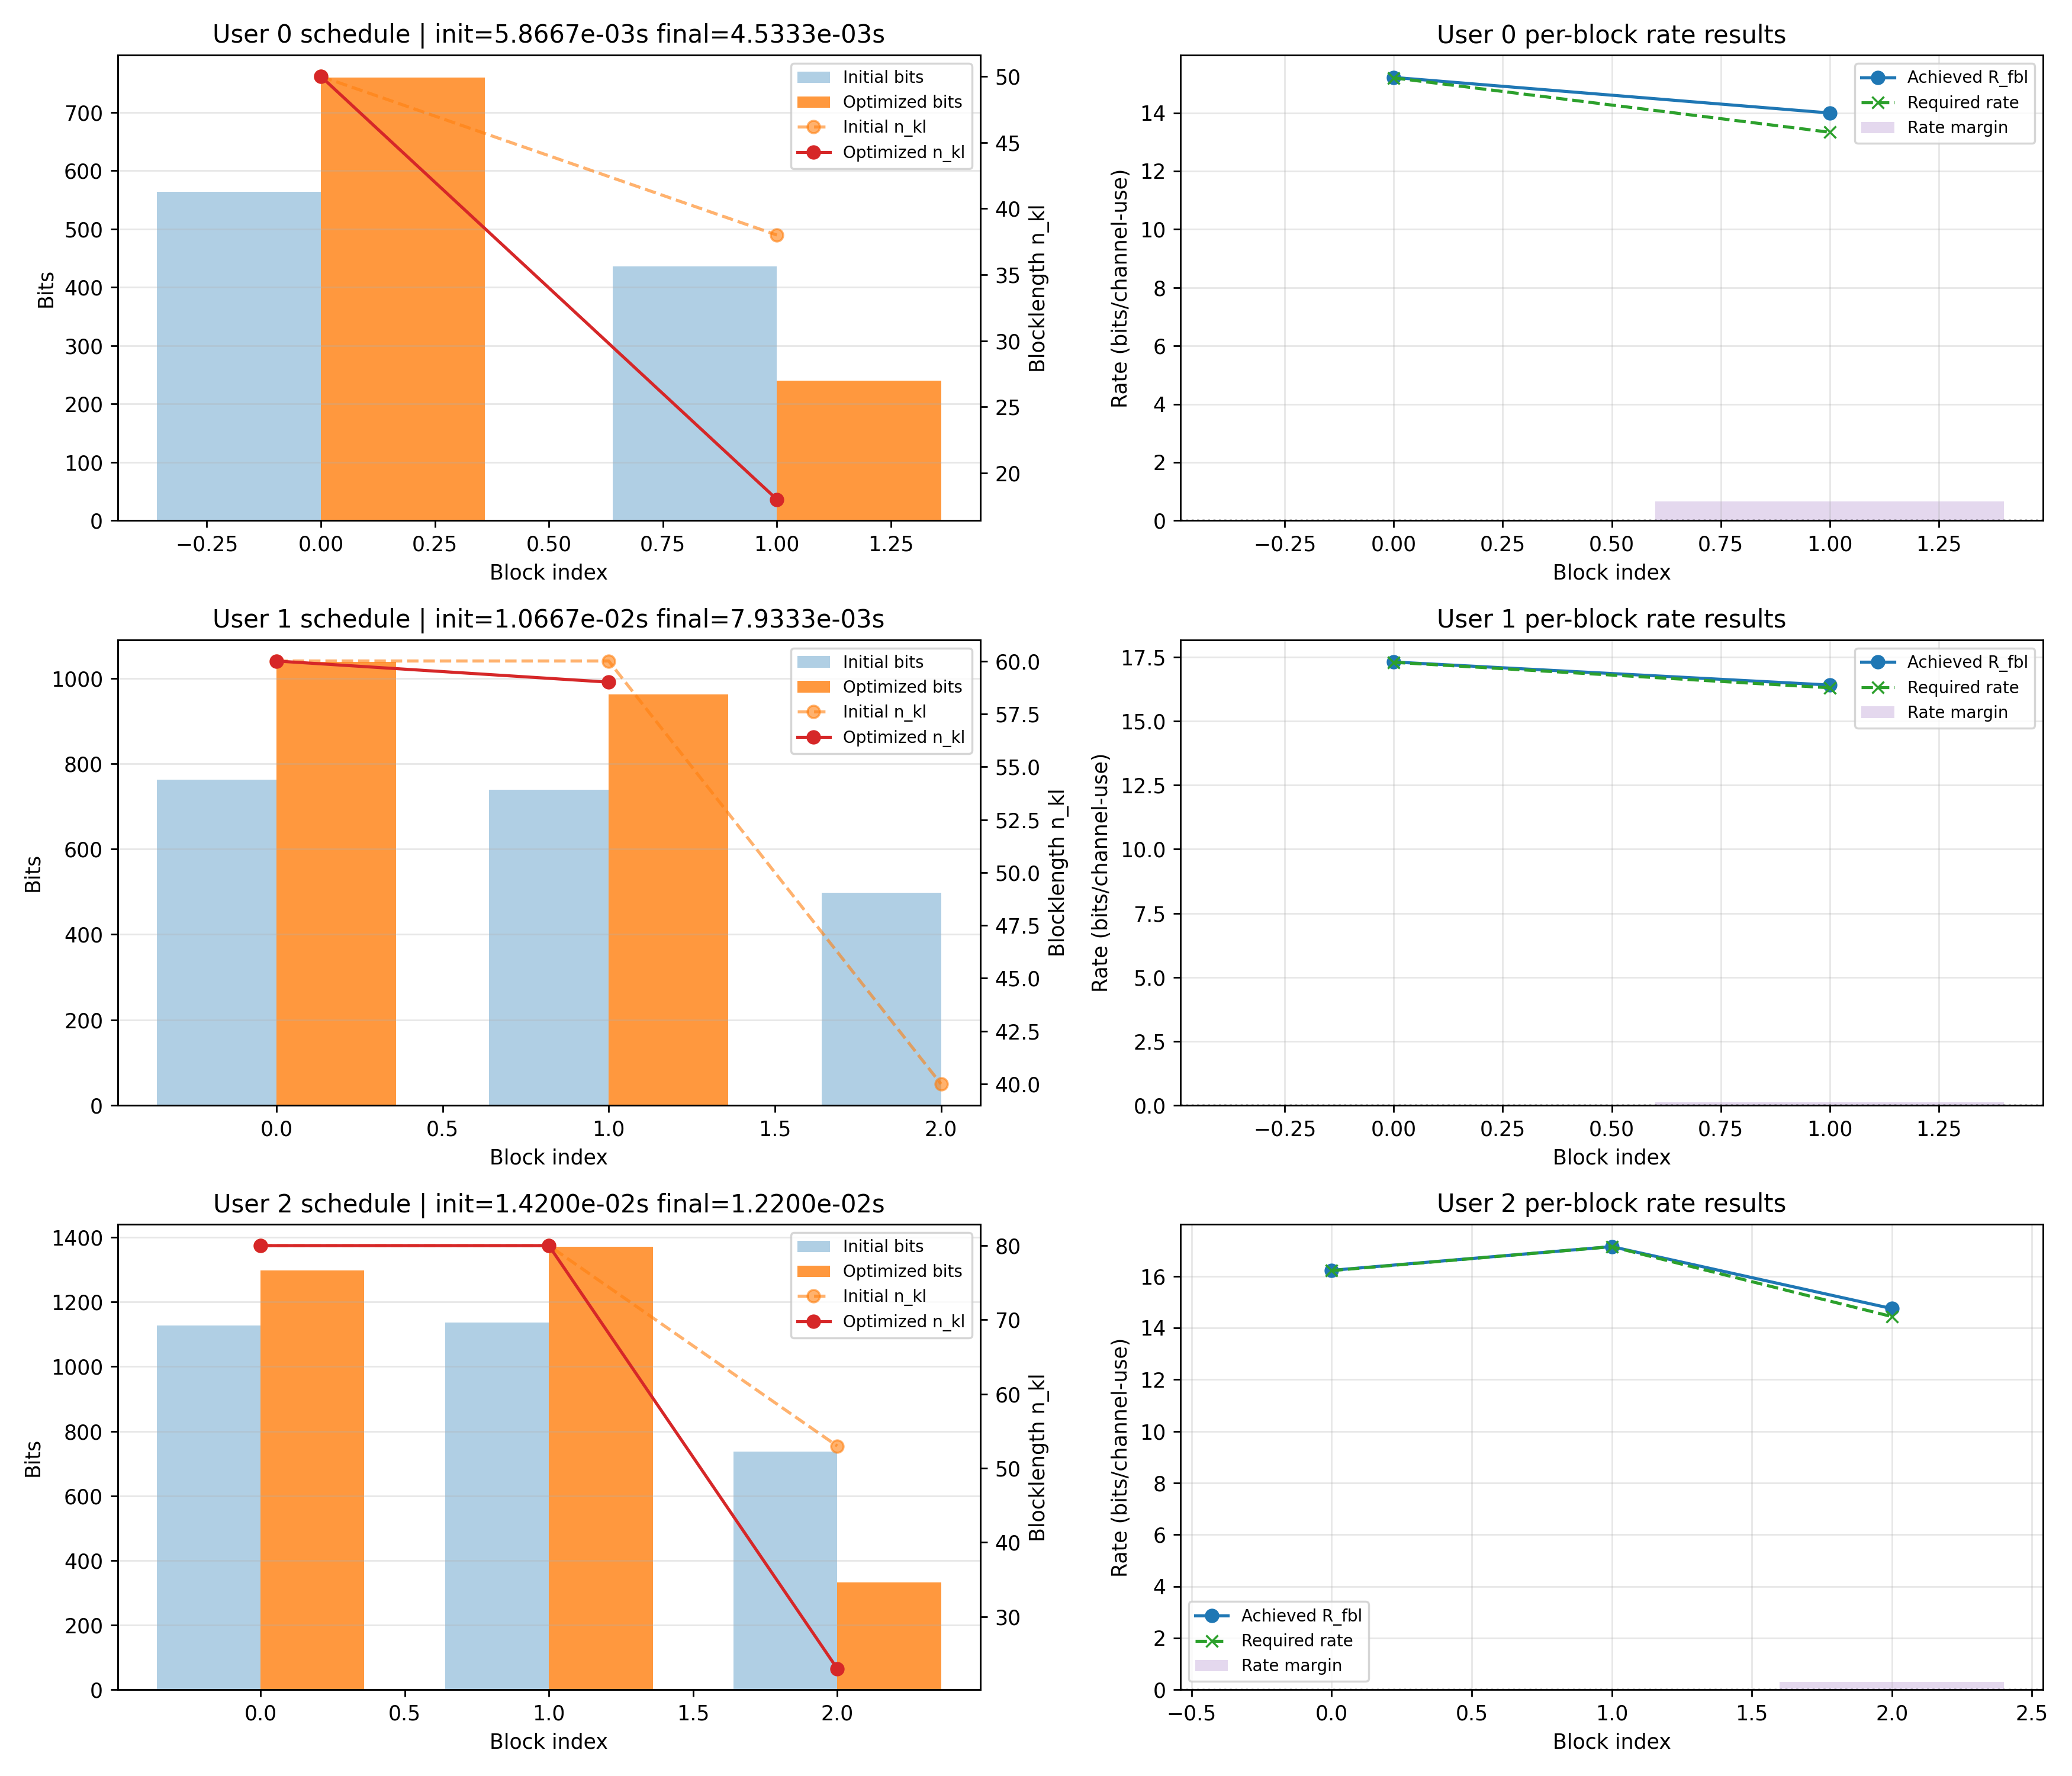
\includegraphics[width=\textwidth,height=0.25\textheight,keepaspectratio]{20260728_ul_per_user_schedule_details_training_only_unweighted.png}
    \caption{Training Only Method, unweighted}
\end{subfigure}
\hfill
\begin{subfigure}[t]{0.48\textwidth}
    \centering
    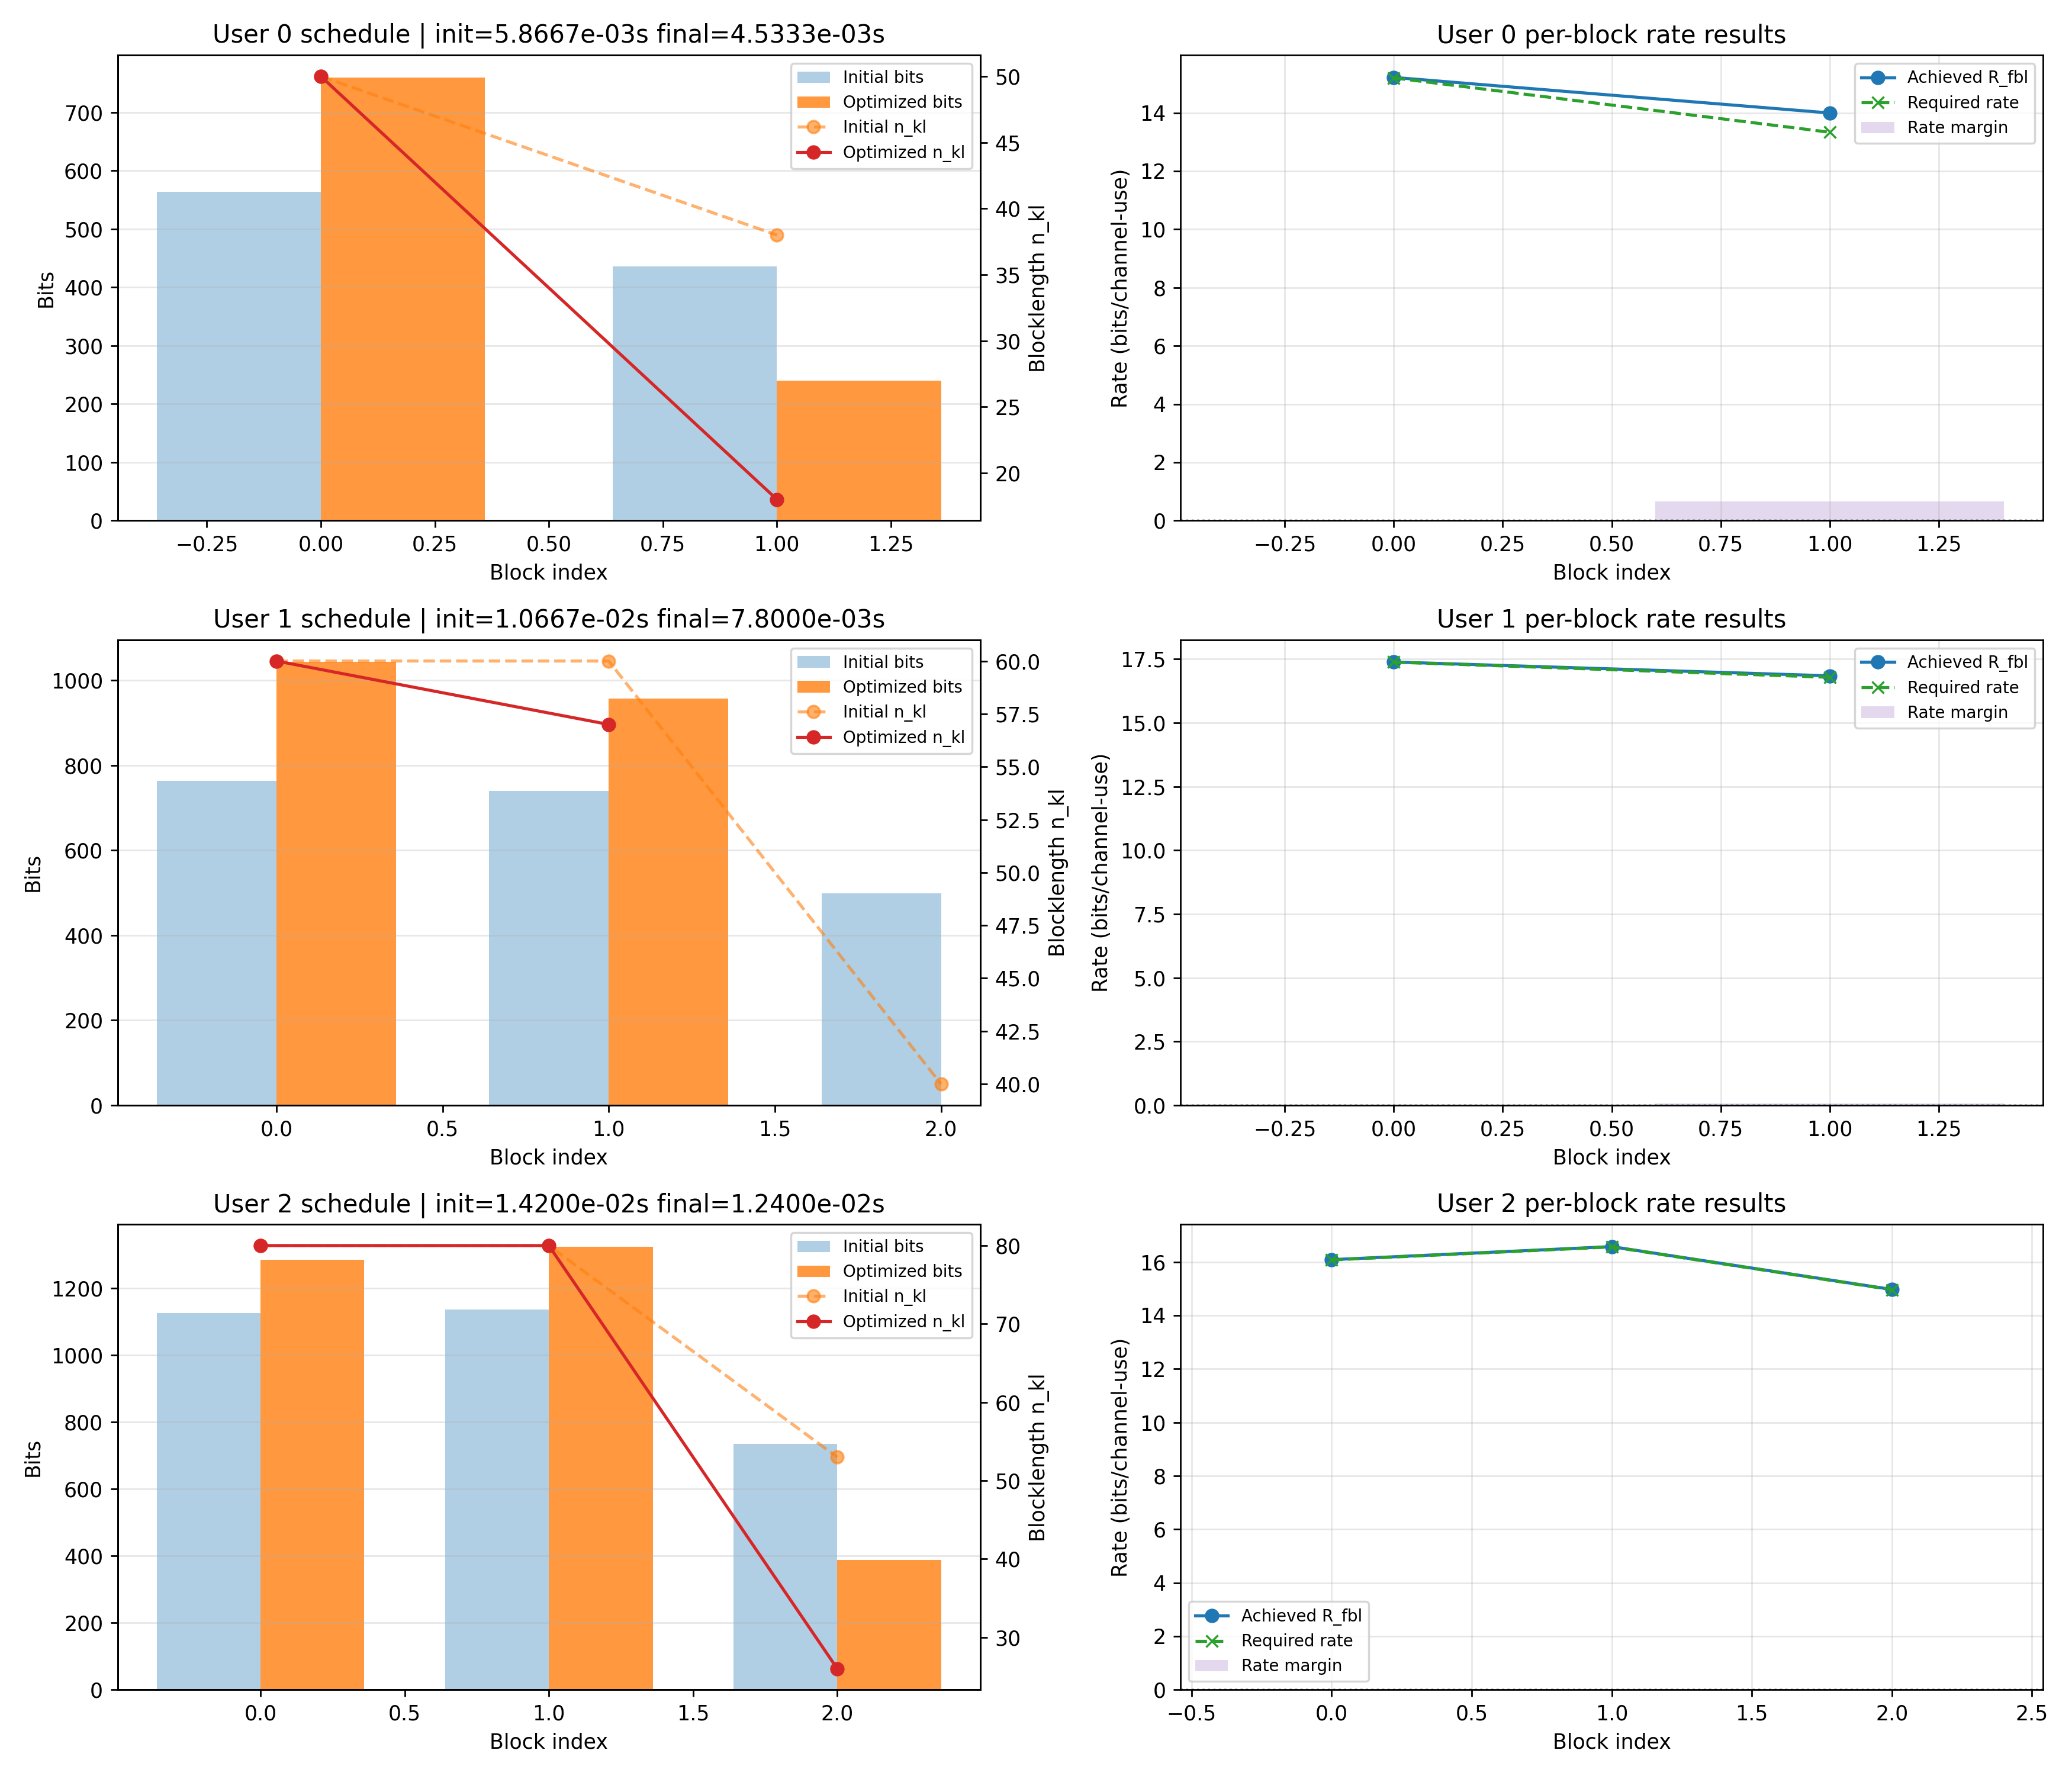
\includegraphics[width=\textwidth,height=0.25\textheight,keepaspectratio]{20260728_ul_per_user_schedule_details_training_only_invcnr.png}
    \caption{Training Only Method, inverse-CNR-weighted}
\end{subfigure}

\vspace{0.5em}

\begin{subfigure}[t]{0.48\textwidth}
    \centering
    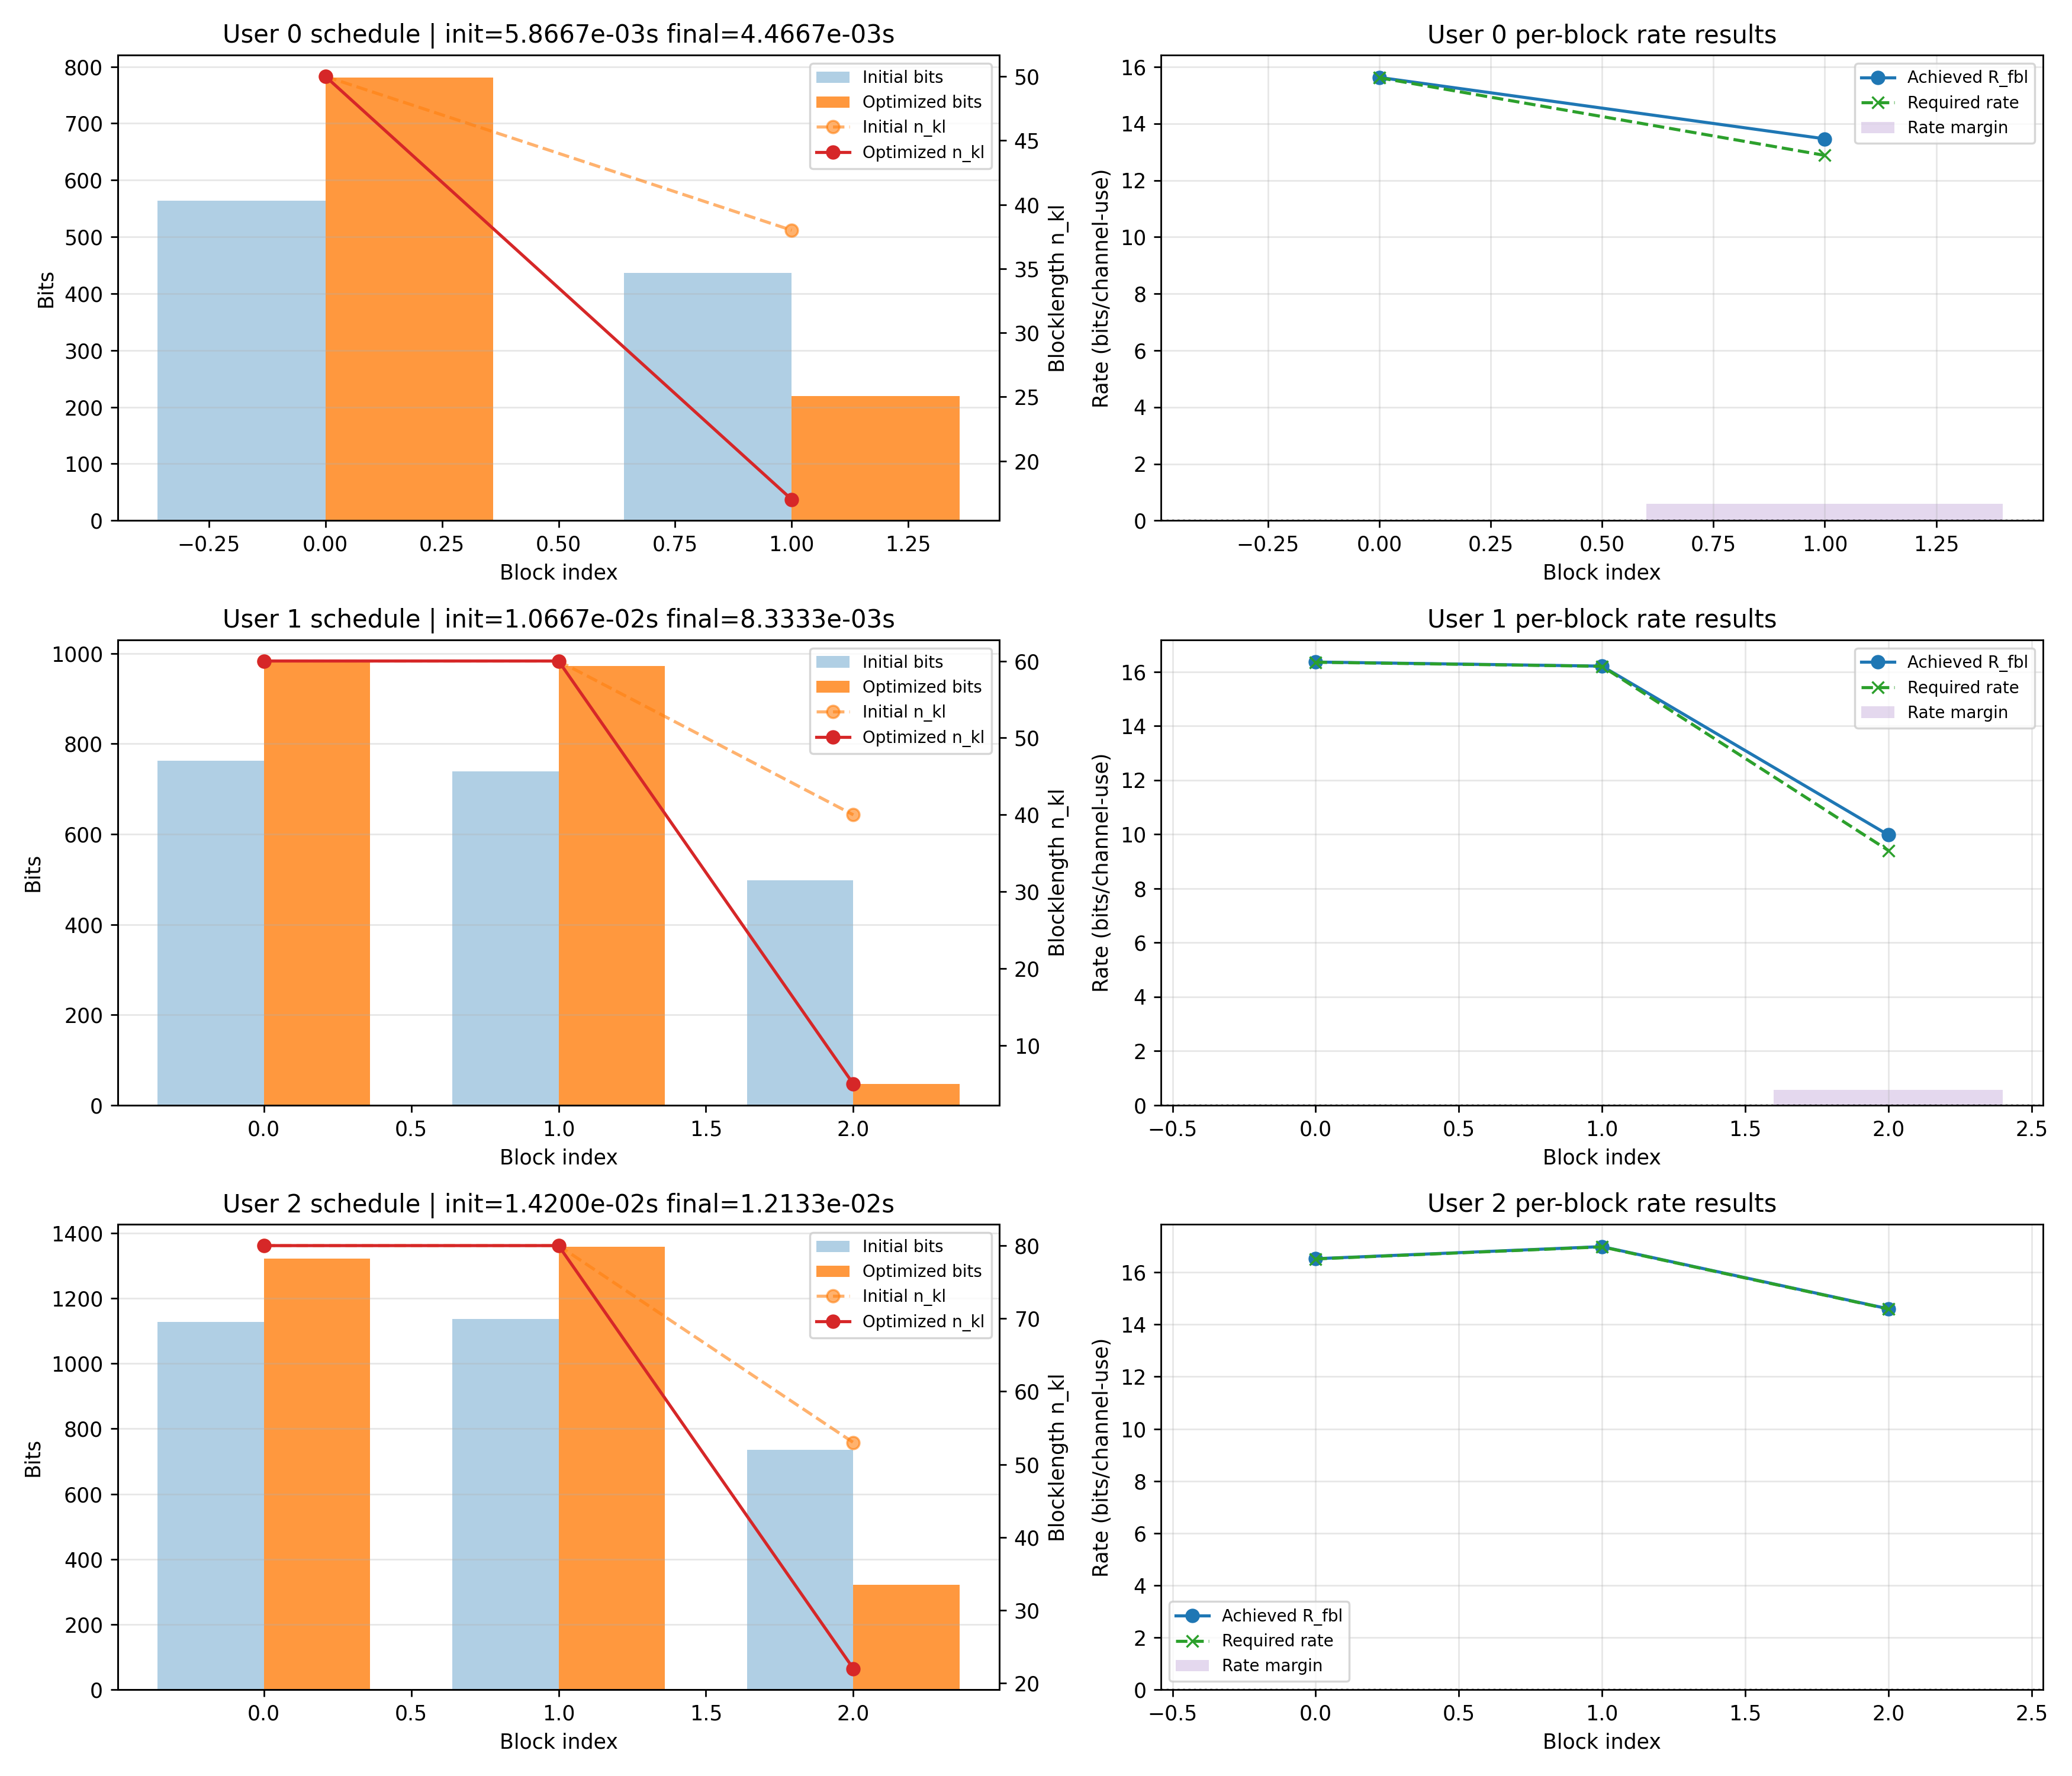
\includegraphics[width=\textwidth,height=0.25\textheight,keepaspectratio]{20260728_ul_per_user_schedule_details_training_testing_unweighted.png}
    \caption{Training + Testing Method, unweighted}
\end{subfigure}
\hfill
\begin{subfigure}[t]{0.48\textwidth}
    \centering
    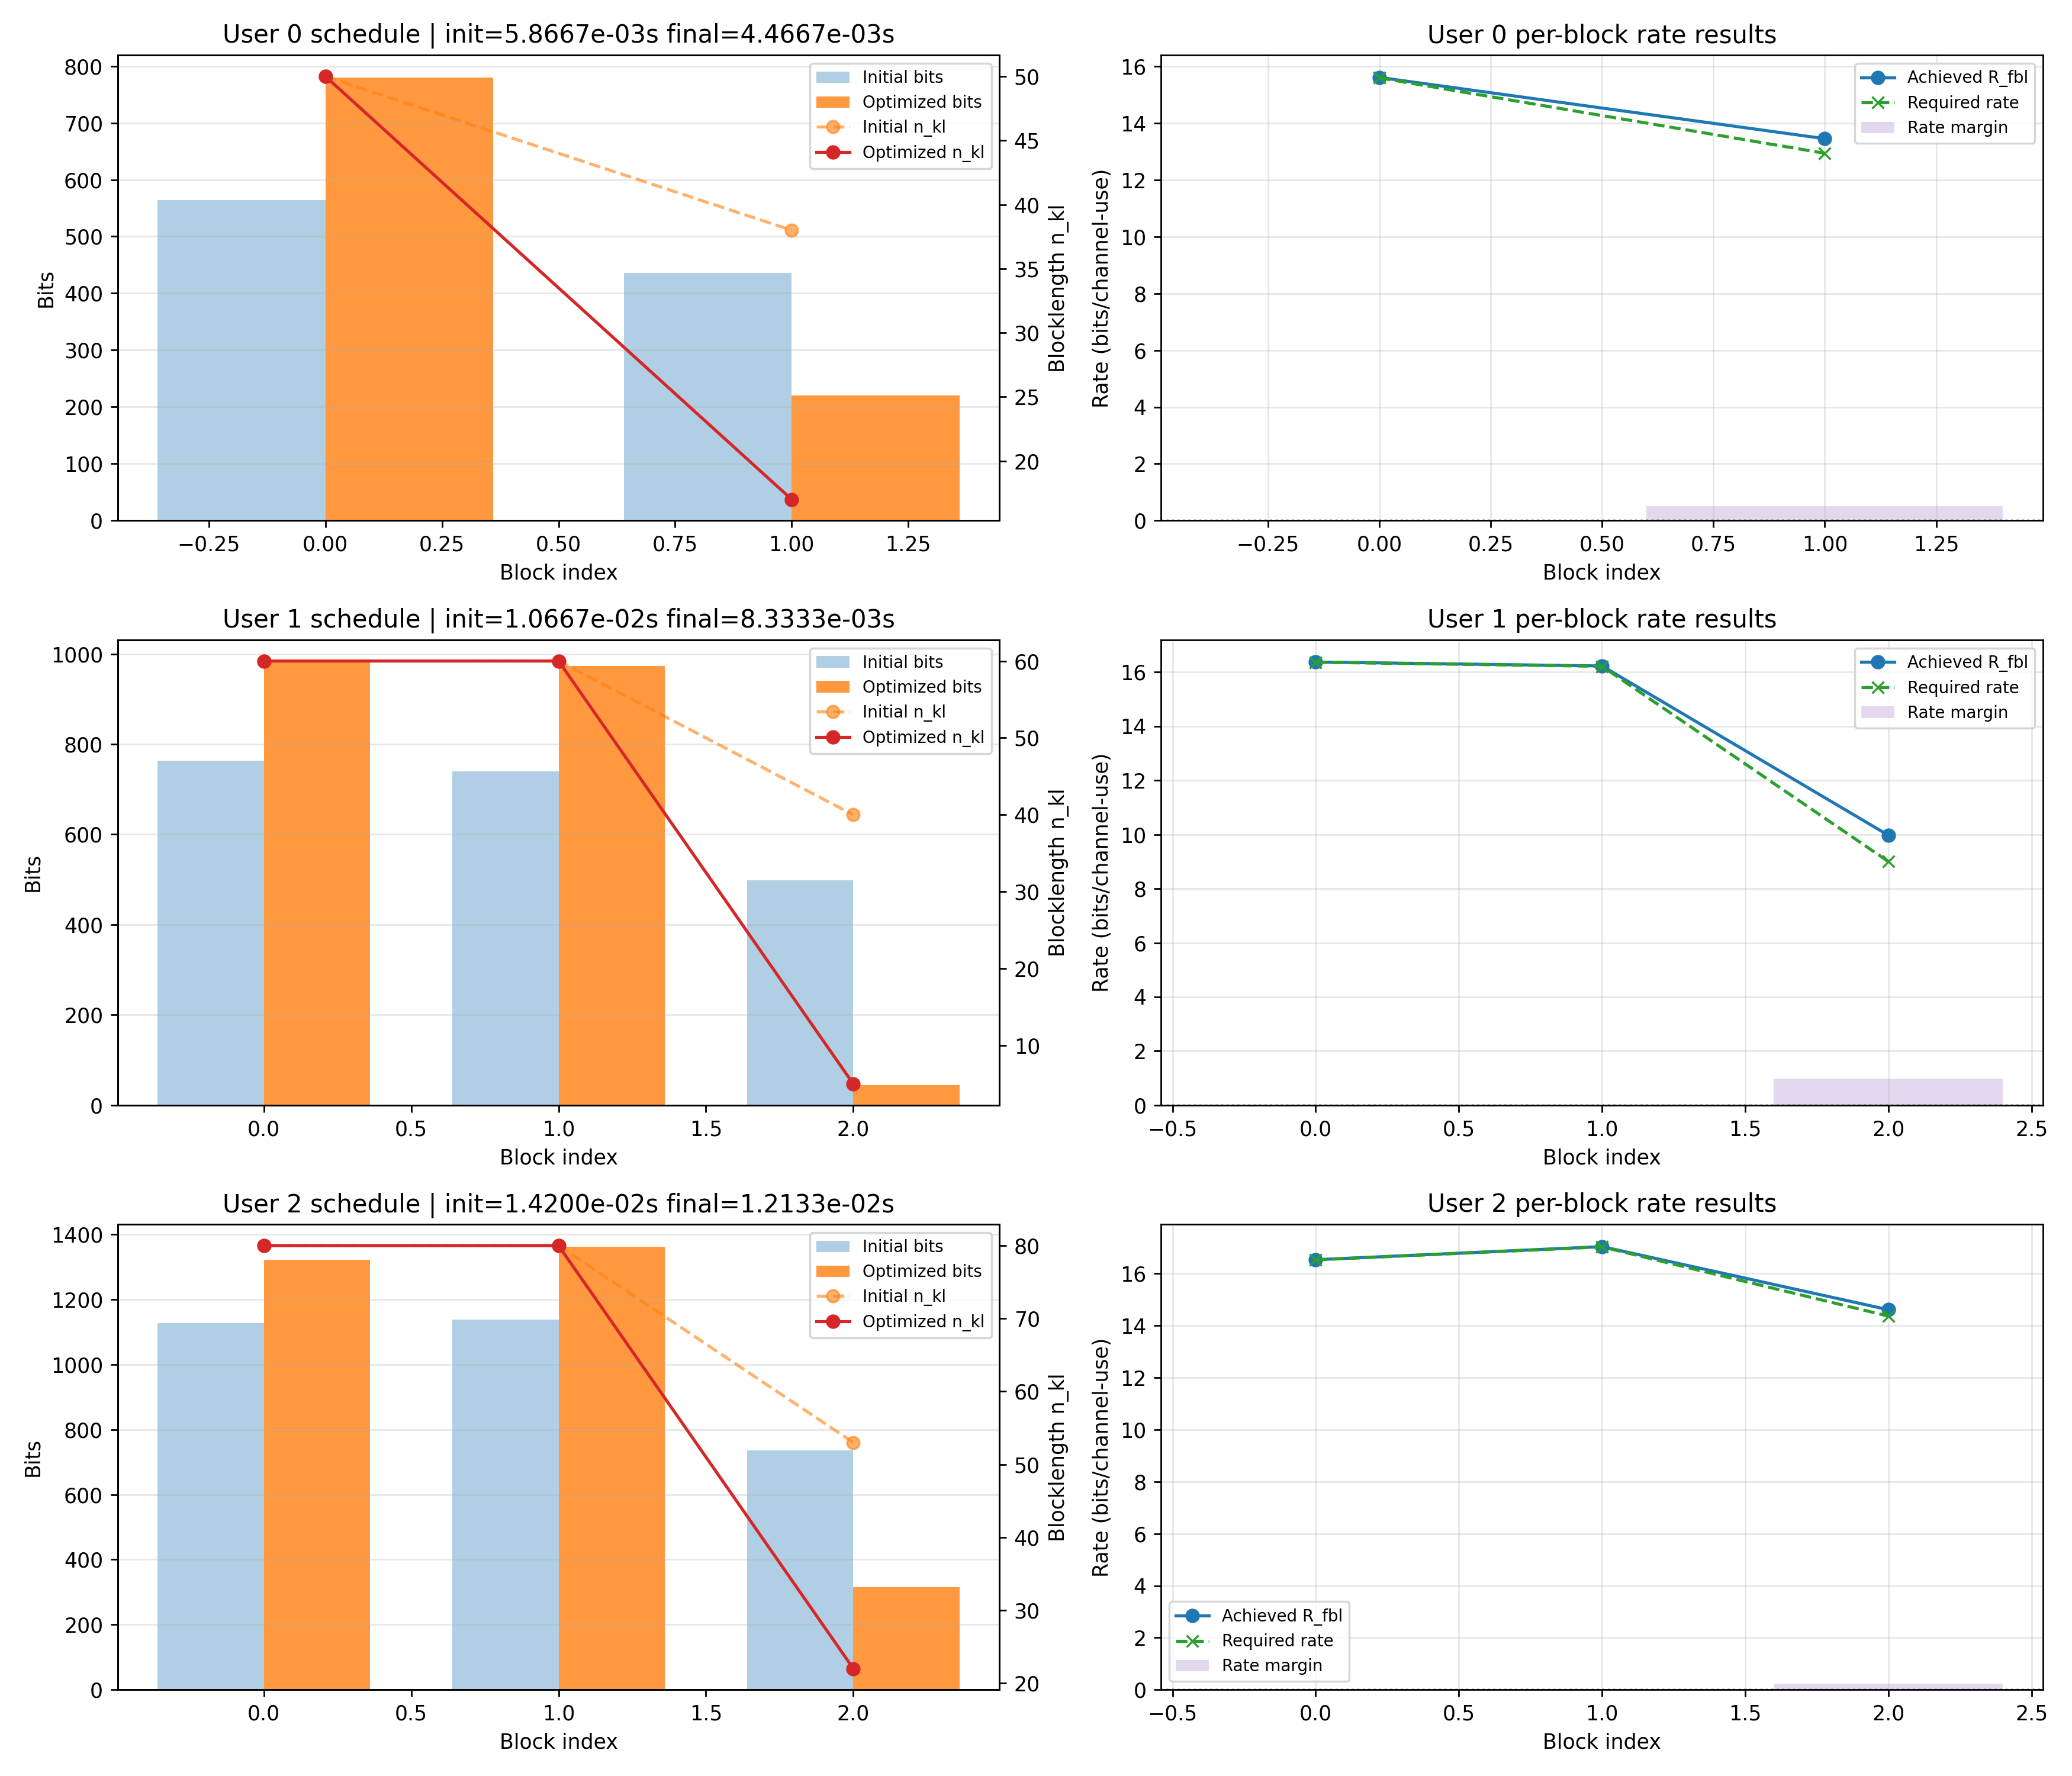
\includegraphics[width=\textwidth,height=0.25\textheight,keepaspectratio]{20260728_ul_per_user_schedule_details_training_testing_invcnr.png}
    \caption{Training + Testing Method, inverse-CNR-weighted}
\end{subfigure}
\caption{Uplink per-user schedule details for the unweighted and inverse-CNR-weighted objectives. The benchmark changes only slightly under weighting, and the \emph{Training + Testing Method} keeps the same overall schedule shape in both modes.}
\label{fig:uplink-objective-schedules}
\end{figure}

\section{Downlink}

The downlink reacts more strongly to the objective choice. In the benchmark,
inverse-CNR weighting shortens the schedule tail by collapsing user 2 from four
blocks to two and reducing its total assigned sub-blocklength from \(260\) to
\(147\). In the \emph{Training + Testing Method}, the weighted run still has a
longer schedule than the benchmark, but it improves both total latency and
asynchronality relative to the unweighted case.

\begin{table}[H]
\centering
\scriptsize
\setlength{\tabcolsep}{3pt}
\renewcommand{\arraystretch}{1.12}
\begin{tabularx}{\textwidth}{>{\raggedright\arraybackslash}p{0.24\textwidth} *{4}{>{\raggedright\arraybackslash}X}}
\toprule
Metric & \shortstack{Training\\Only\\Unweighted} & \shortstack{Training\\Only\\Inv.-CNR} & \shortstack{Training +\\Testing\\Unweighted} & \shortstack{Training +\\Testing\\Inv.-CNR} \\
\midrule
Blocks / user & 5, 4, 4 & 5, 4, 2 & 9, 3, 7 & 9, 7, 4 \\
Total $n$ / user & 248, 232, 260 & 248, 209, 147 & 437, 168, 530 & 436, 395, 273 \\
Skipped blocks / user & 4, 0, 0 & 4, 2, 0 & 7, 0, 3 & 7, 4, 0 \\
\addlinespace
Init. total & 0.305000 & 0.305000 & 0.305000 & 0.305000 \\
Final total & 0.049333 & 0.040267 & 0.075667 & 0.073600 \\
Red. (\%) & 83.8251 & 86.7978 & 75.1913 & 75.8689 \\
\addlinespace
Init. avg & 0.101667 & 0.101667 & 0.101667 & 0.101667 \\
Final avg & 0.016444 & 0.013422 & 0.025222 & 0.024533 \\
\addlinespace
Init. async. & 0.131600 & 0.131600 & 0.131600 & 0.131600 \\
Final async. & 0.003733 & 0.013467 & 0.048267 & 0.021733 \\
Async. red. (\%) & 97.1631 & 89.7670 & 63.3232 & 83.4853 \\
\addlinespace
Init. SNR (dB) & 8.0000 & 8.0000 & 8.0000 & 8.0000 \\
Final SNR (dB) & 14.1792 & 15.3203 & 9.3594 & 9.8556 \\
\addlinespace
Init. SINR (dB) & -2.8373 & -2.8373 & -2.8373 & -2.8373 \\
Final SINR (dB) & 8.2492 & 18.6234 & 11.9746 & 13.0376 \\
\bottomrule
\end{tabularx}
\caption{Downlink payload-completion summary for the unweighted and inverse-CNR-weighted objectives.}
\label{tab:downlink-objective-schedule-summary}
\end{table}

\begin{figure}[H]
\centering
\begin{subfigure}[t]{0.48\textwidth}
    \centering
    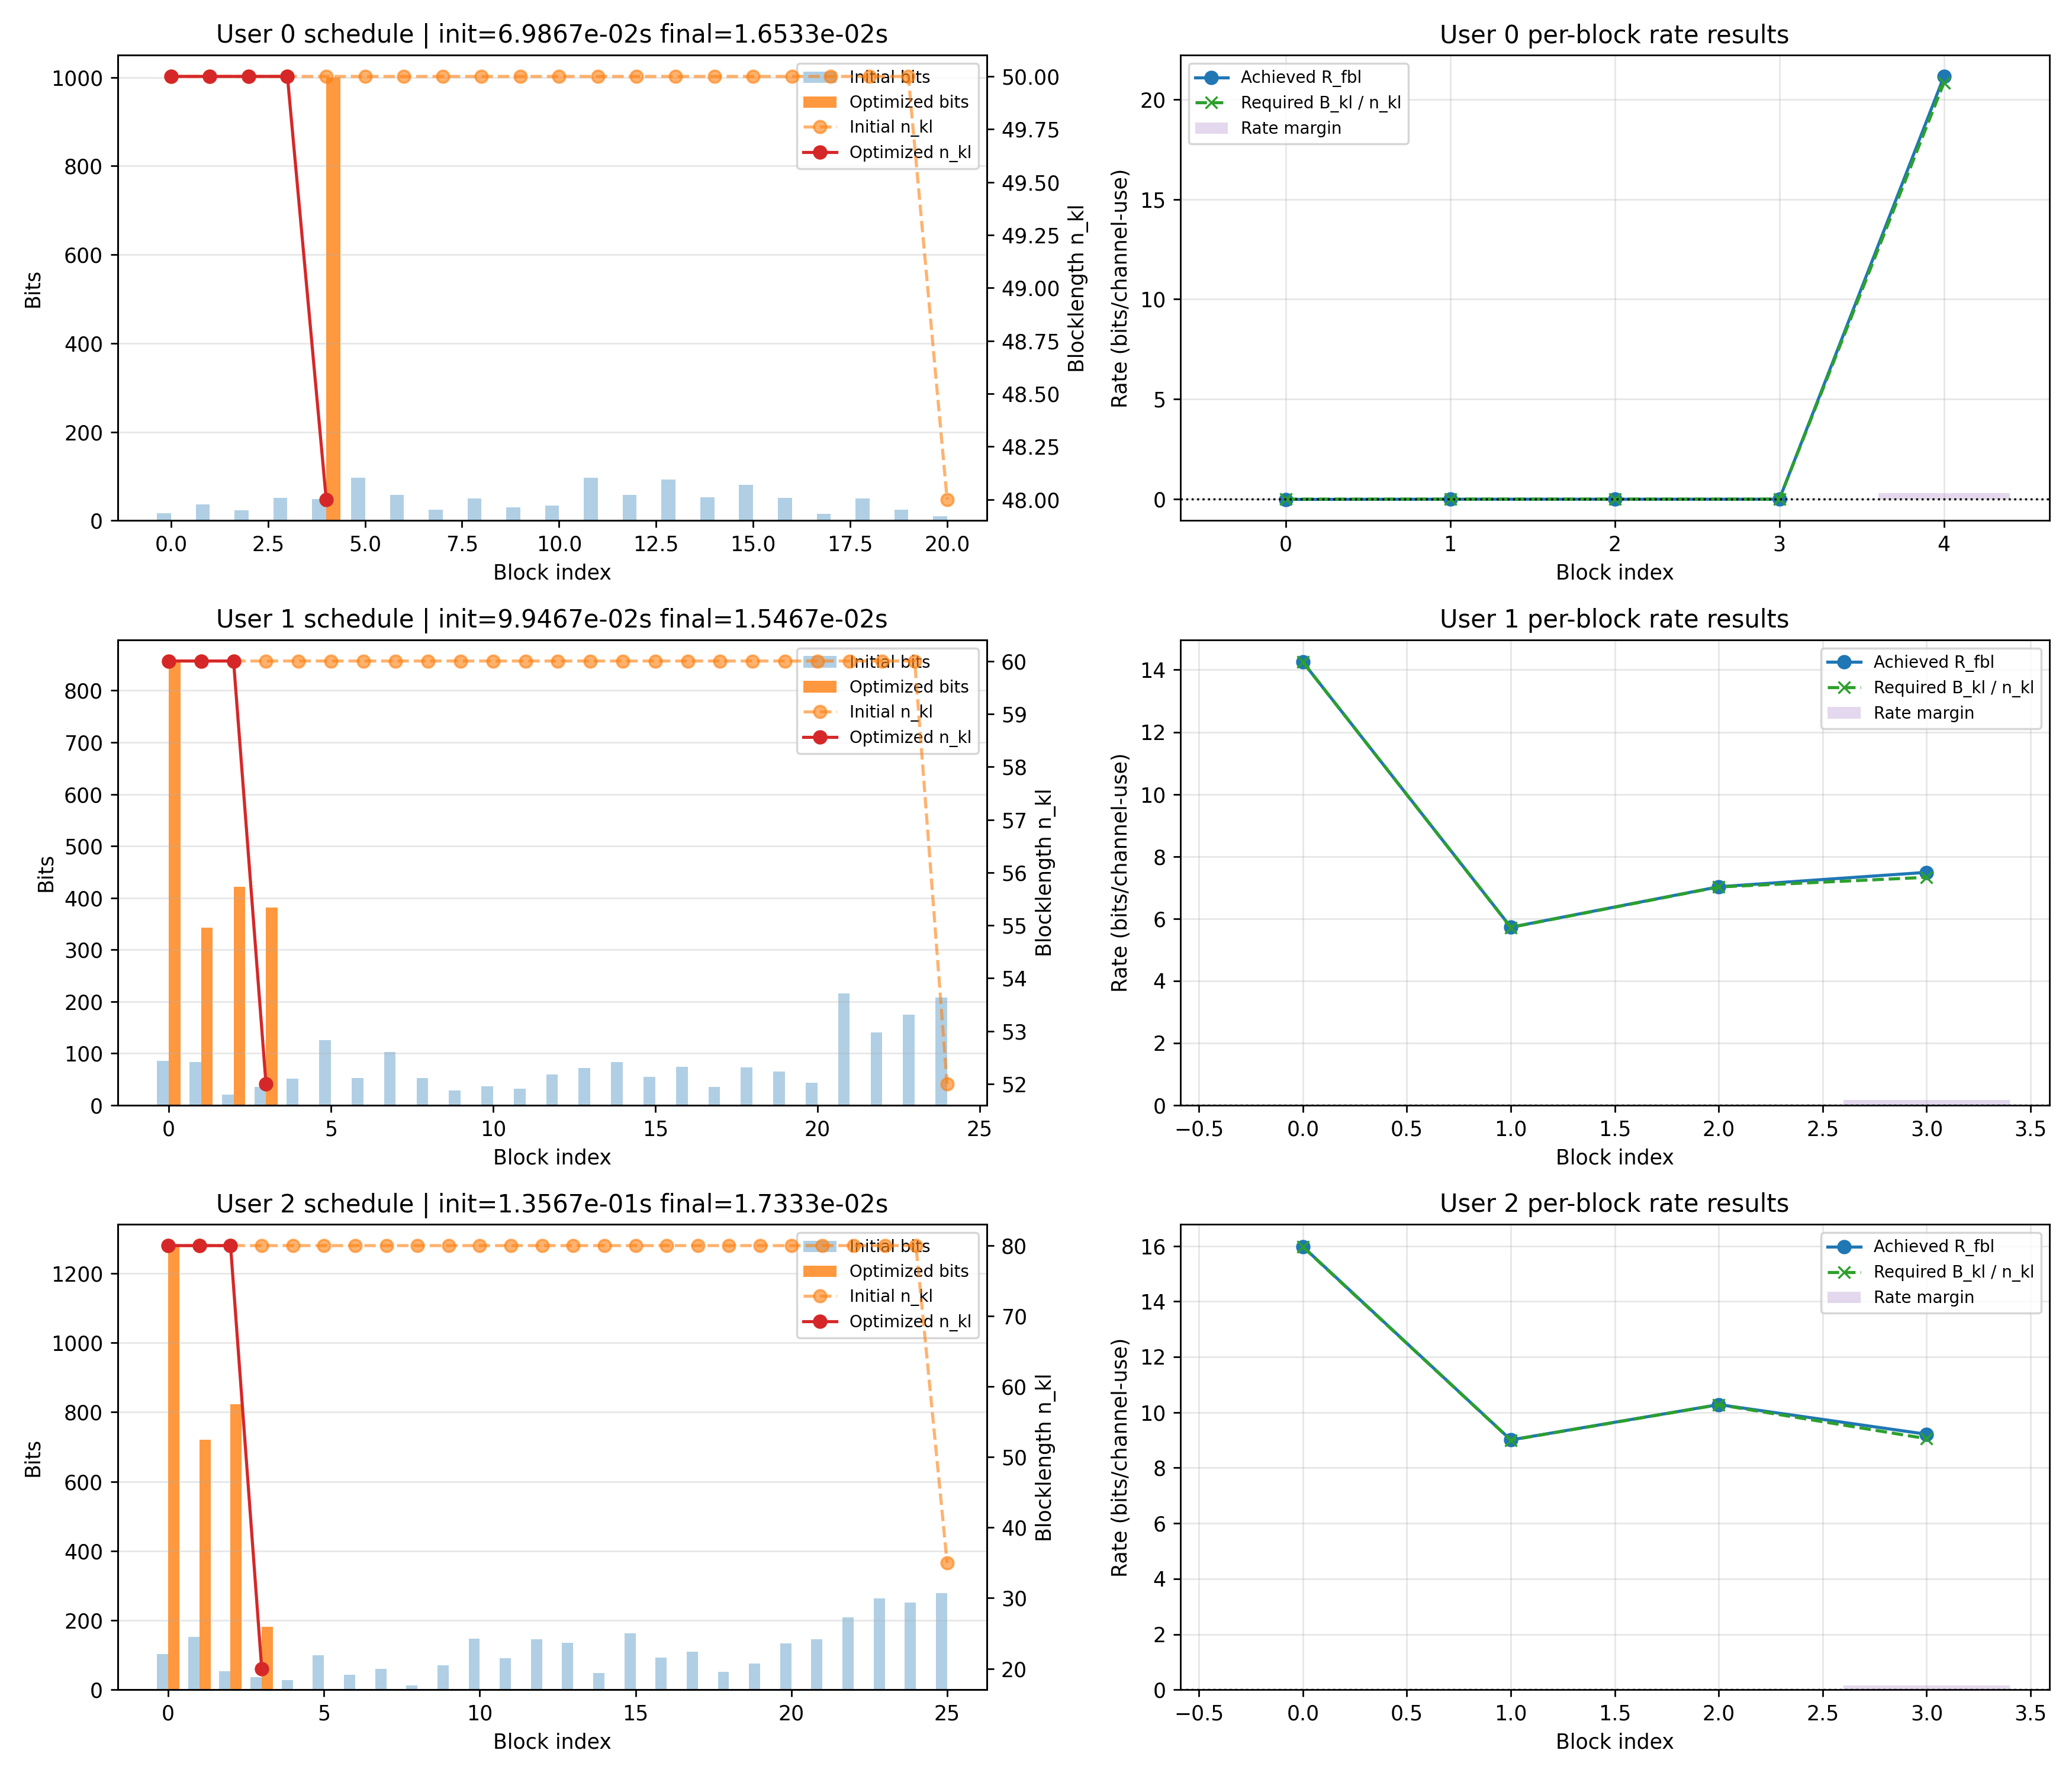
\includegraphics[width=\textwidth,height=0.25\textheight,keepaspectratio]{20260728_dl_per_user_schedule_details_training_only_unweighted.png}
    \caption{Training Only Method, unweighted}
\end{subfigure}
\hfill
\begin{subfigure}[t]{0.48\textwidth}
    \centering
    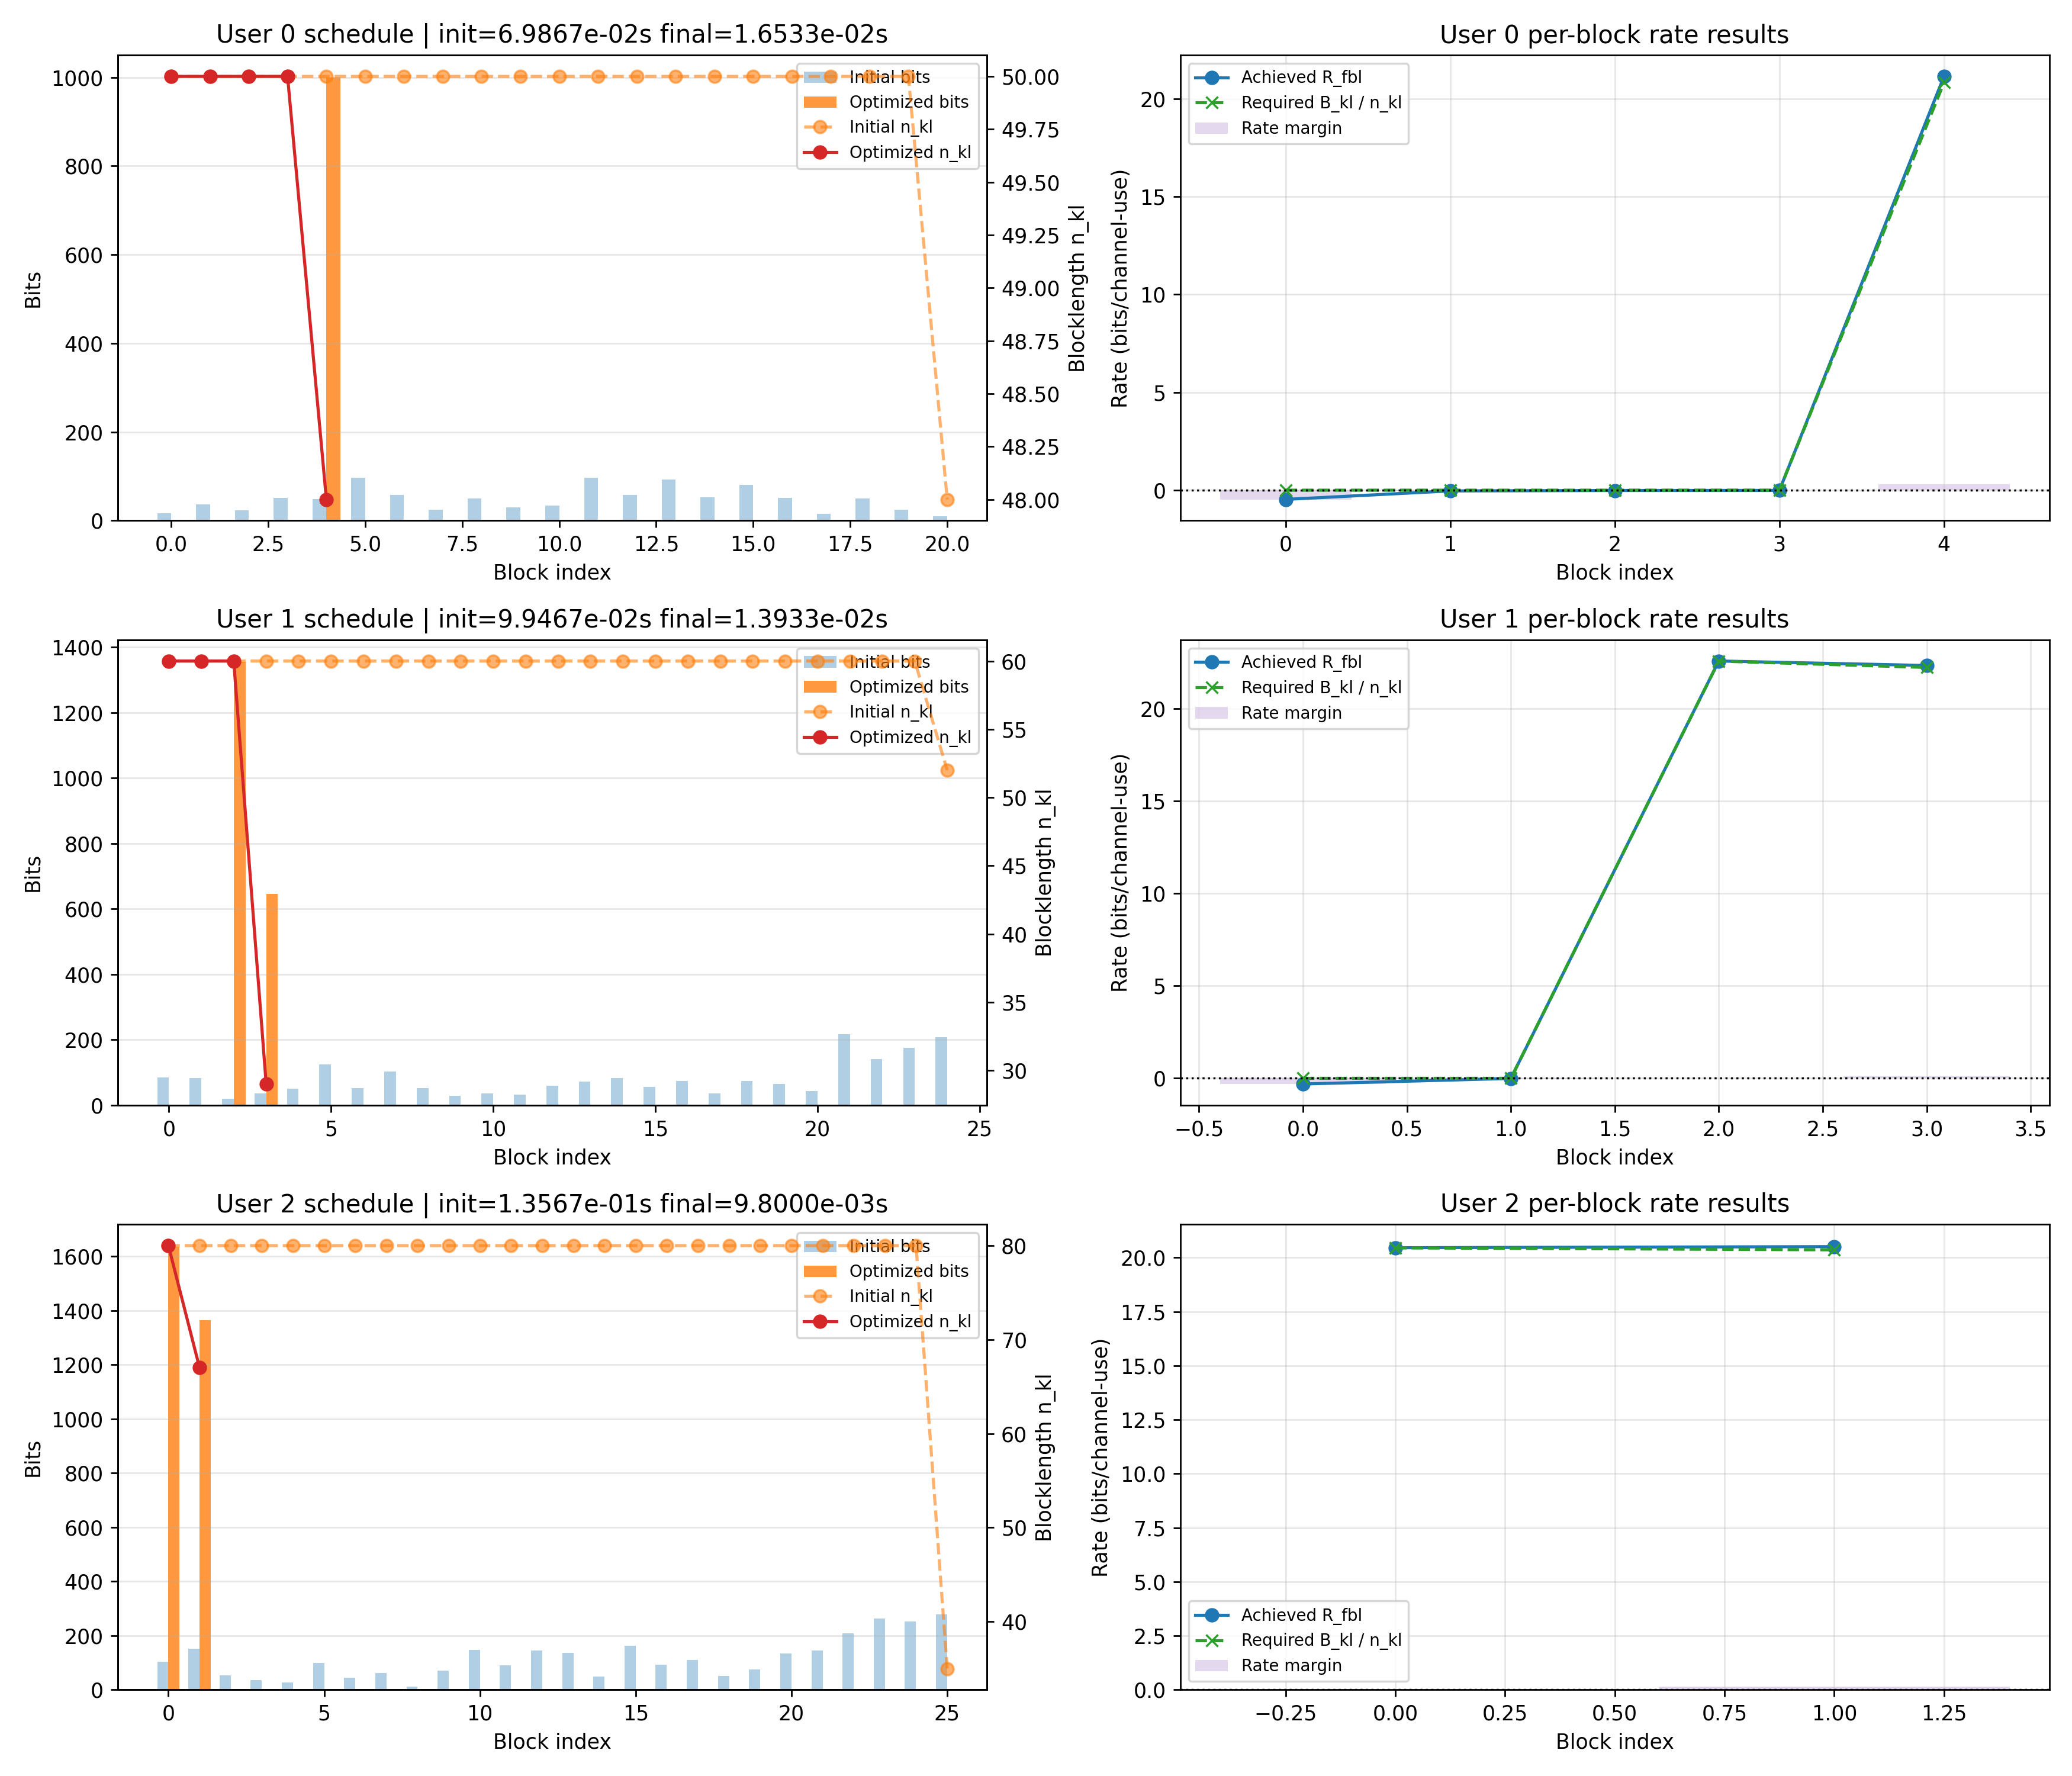
\includegraphics[width=\textwidth,height=0.25\textheight,keepaspectratio]{20260728_dl_per_user_schedule_details_training_only_invcnr.png}
    \caption{Training Only Method, inverse-CNR-weighted}
\end{subfigure}

\vspace{0.5em}

\begin{subfigure}[t]{0.48\textwidth}
    \centering
    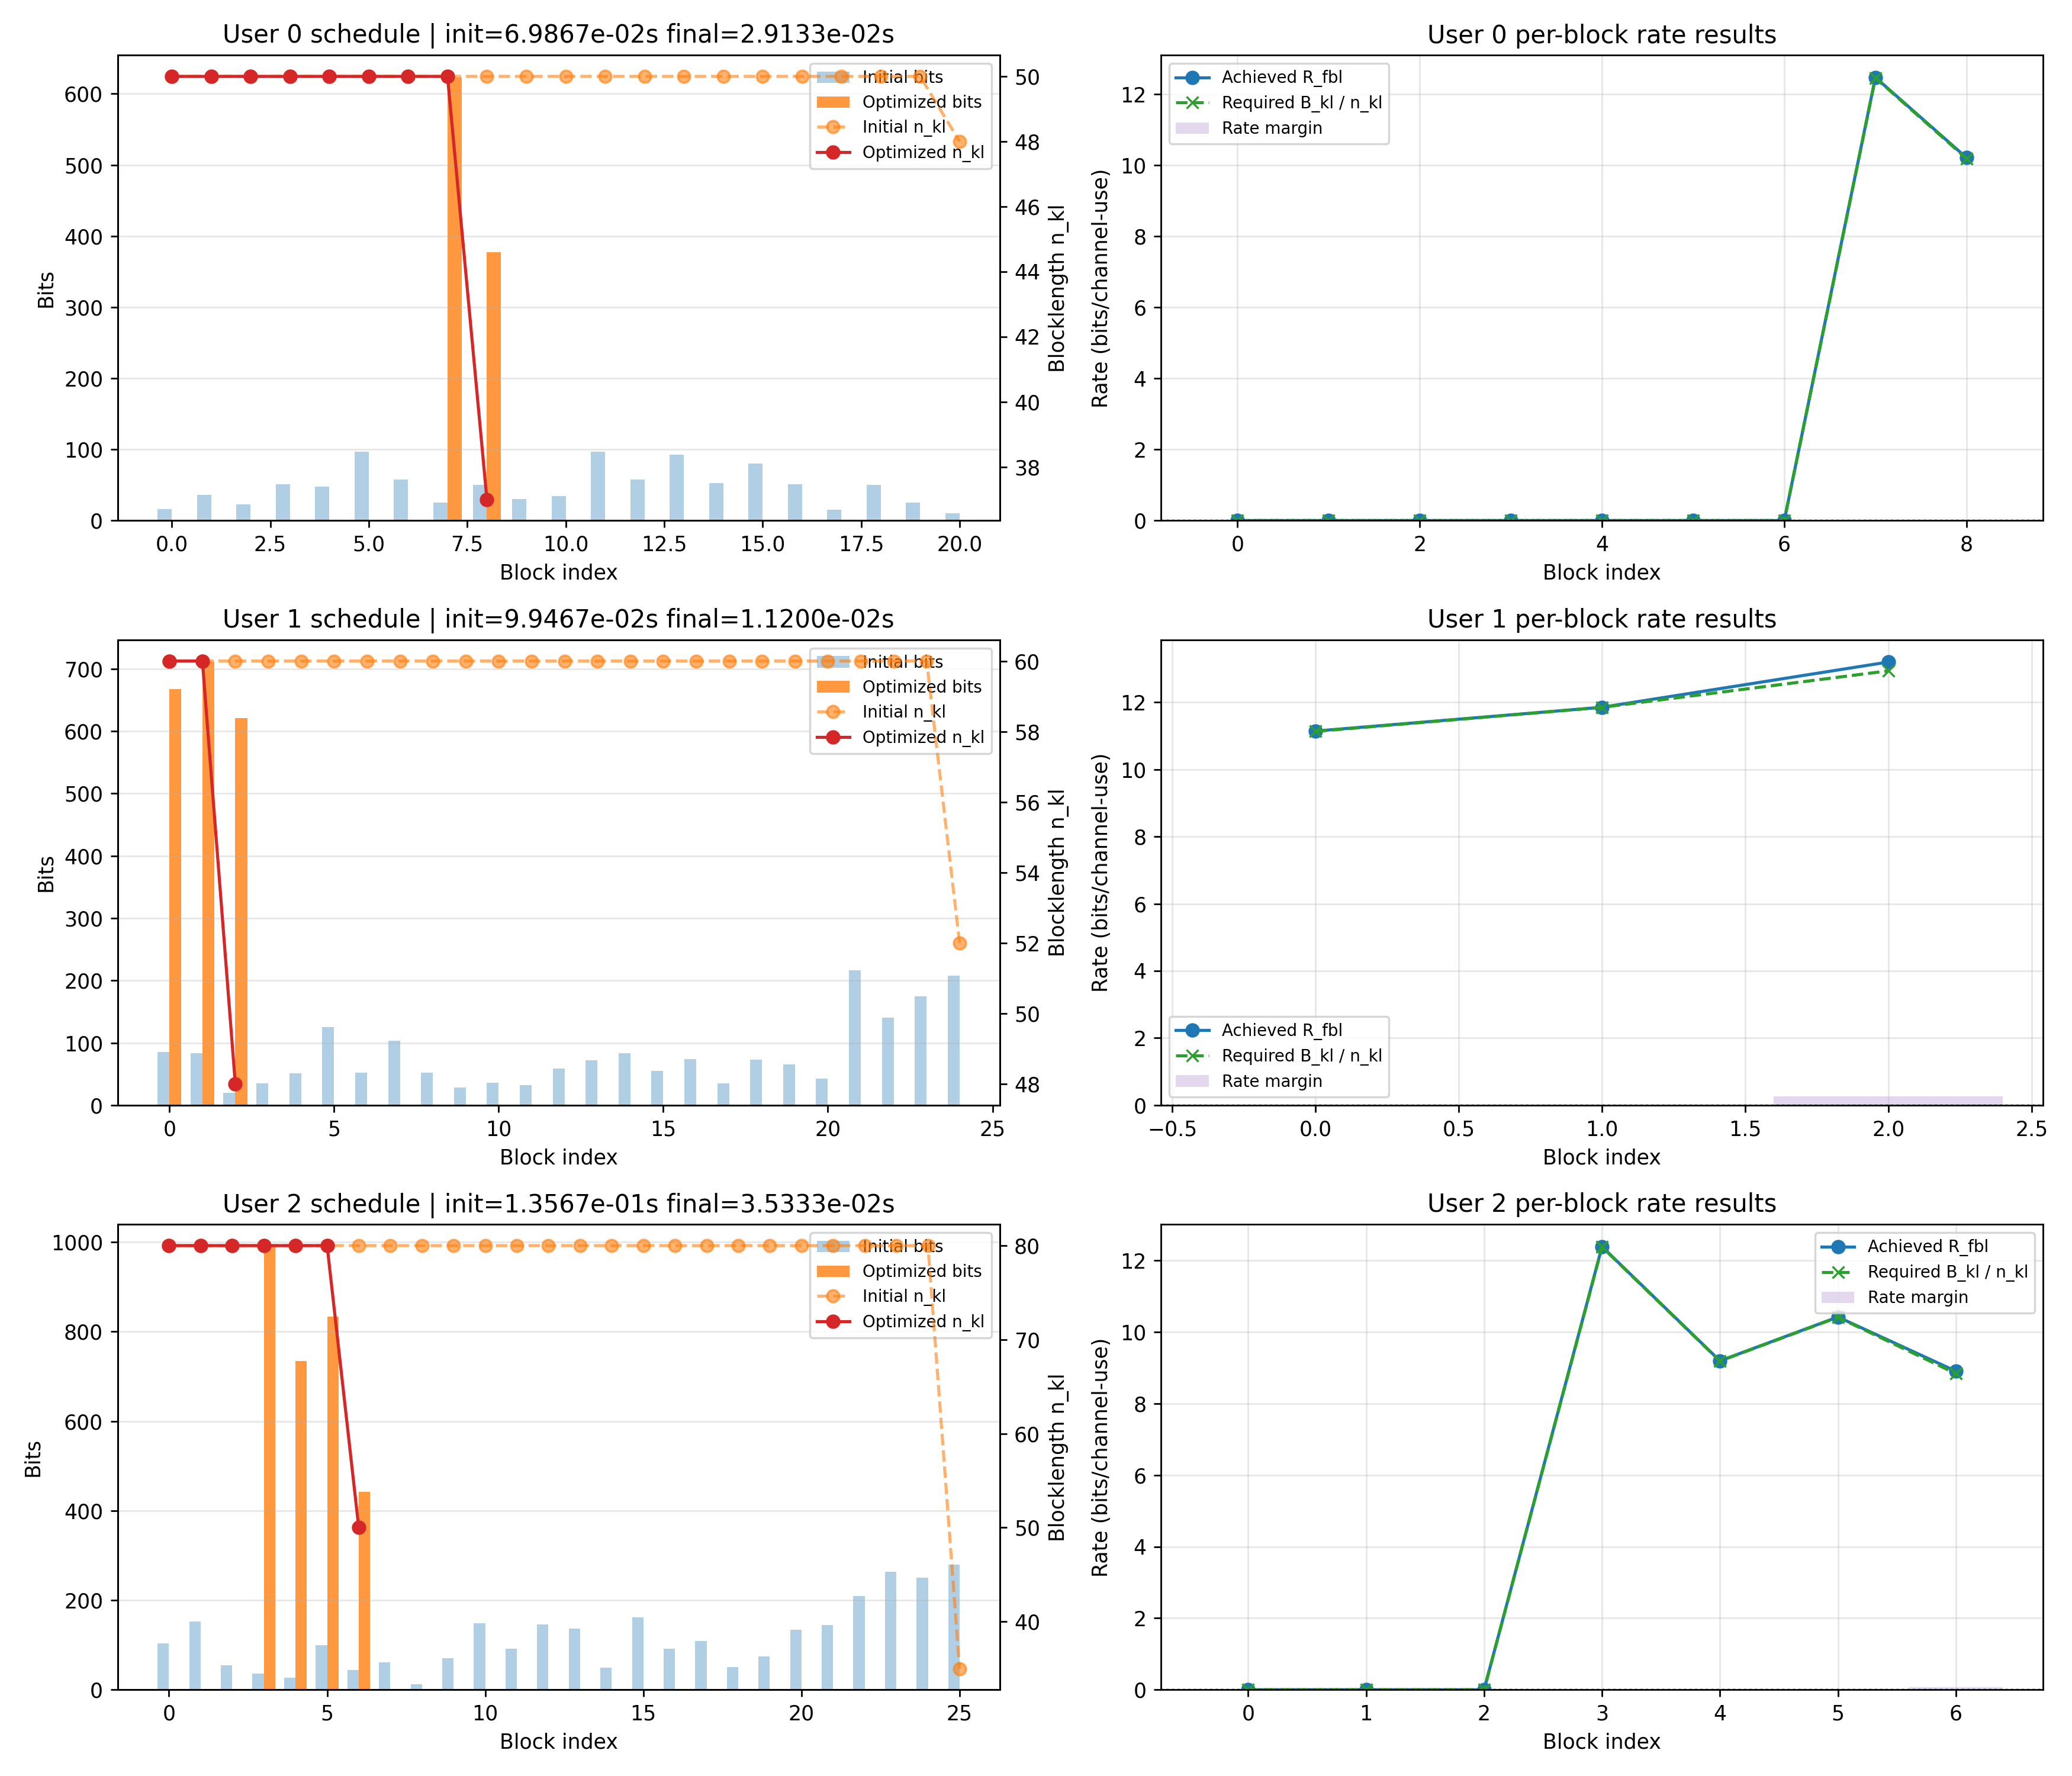
\includegraphics[width=\textwidth,height=0.25\textheight,keepaspectratio]{20260728_dl_per_user_schedule_details_training_testing_unweighted.png}
    \caption{Training + Testing Method, unweighted}
\end{subfigure}
\hfill
\begin{subfigure}[t]{0.48\textwidth}
    \centering
    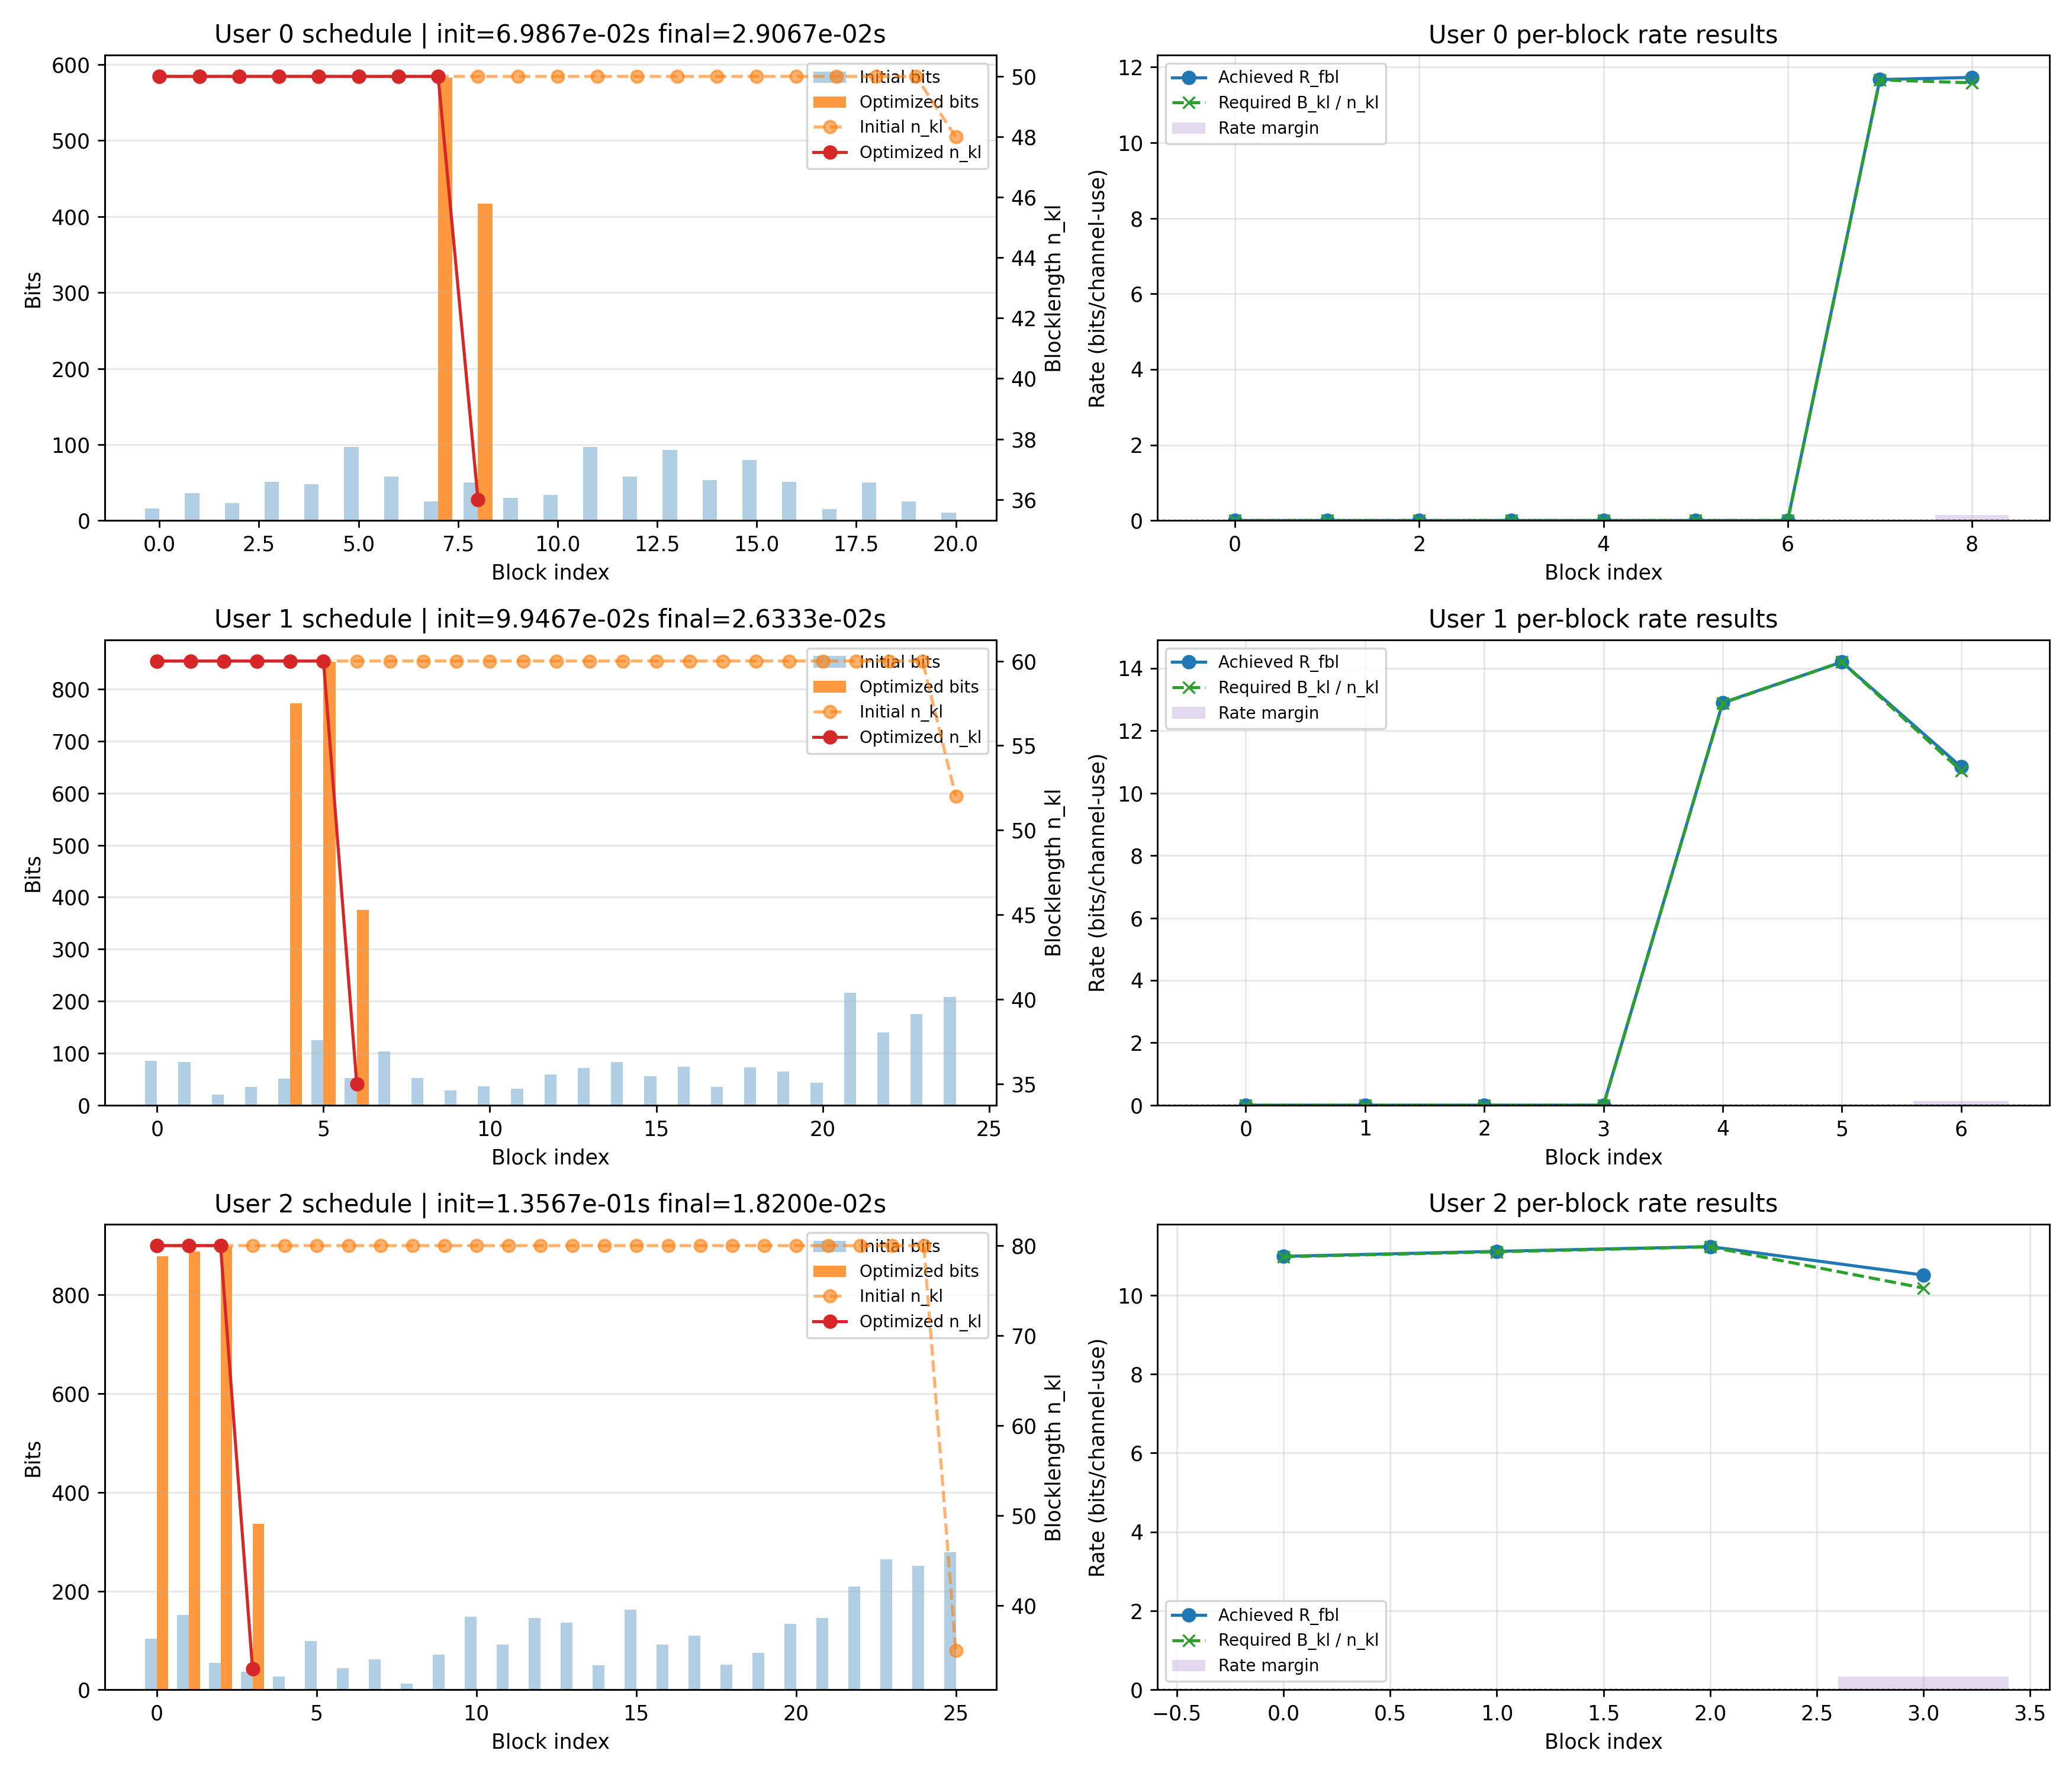
\includegraphics[width=\textwidth,height=0.25\textheight,keepaspectratio]{20260728_dl_per_user_schedule_details_training_testing_invcnr.png}
    \caption{Training + Testing Method, inverse-CNR-weighted}
\end{subfigure}
\caption{Downlink per-user schedule details for the unweighted and inverse-CNR-weighted objectives. The weighted benchmark becomes visibly shorter on user 2, while the weighted \emph{Training + Testing Method} improves over the unweighted case but remains more fragmented than the benchmark.}
\label{fig:downlink-objective-schedules}
\end{figure}

\section{Schedule Takeaways}

In the uplink, inverse-CNR weighting changes the benchmark only marginally and
does not change the \emph{Training + Testing Method} schedule pattern at all.
So the uplink objective comparison is mostly a fine redistribution effect rather
than a structural scheduling shift.

In the downlink, the objective choice matters more. The benchmark benefits most
clearly in final latency, while the \emph{Training + Testing Method} gains both
lower total latency and better synchronization under inverse-CNR weighting.

\end{document}
